\subsection{Resilient Distributed Datasets}
Major methods in Spark are Resilient Distributed Datasets (RDDs), a data structure that abstracts distributed memory across different clusters. 
The immutable coarse-grained transformation, spark-scheduler with lazy-evaluation, and memory management with cacheing achieve computation with fault-tolerance, 
fast execution, and moderate control on memory efficiency \cite{DBLP:conf/nsdi/ZahariaCDDMMFSS12}.

A RDD is essentially a multi-layer Java data structure. A top RDD object references Java array, which intern, references a set of tuple objects. 
The coarse-grained transformations and immutability requires a RDD to be deep-copied to produce a new RDD, but efficiently offers fault tolerance. 
The lost partitions of a RDD can be recomputed in parallel on different nodes rather than rolling back the whole program.

Spark-pipeline consists of sequence of transformations and actions over RDDs. A transformation produces a new RDD from a set of existing RDD. 
An action is method that computes statistics from an RDD. Due to lazy-evaluation nature, transformations do not materialize the newly created RDD. 
Instead, RDD Lineages are created. Lineage is a graph among parent and child RDDs which represents logical execution plan. 
This enhance fault-tolerance and improve ability to optimize execution plan. 

RDDs can be cached in memory for faster access by persist method. Developers can specify a storage level for a persisted RDD, in memory with serialized or deserialized, or on disk. 
Other than persisted RDD, Spark generates a lot of intermediate RDDs during execution. Since RDD is a Java object, they are managed by Garbage Collection (GC) in the JVM. 
However, persisted RDDs are never collected by GC. This GC might cause significant deterioration of performance of Spark, because GC shows heavy overhead when there are a number of objects.


\subsection{Memory Management in Spark}
Spark framework allocates multiple executors, JVMs, that run sequence of transformations and actions. As we describe the previous section, data in Spark is mainly stored as Java objects in memory, 
so that they are allocated on JVM heap and managed by JVM Garbage Collection. The data may form three types \cite{DBLP:journals/pvldb/XuGDWW19}: Cached data, Shuffled data, and Operator-generated data. 

Spark can cache data in memory to reduce disk I/O. This Cached data usually long-lived Java objects and span multiple stages in Spark-pipeline. 
Spark allocates a logical storage space to store the cached data as shown in Figure. After aggregation, Spark generates Shuffled data. Shuffled data is usually long-lived, 
because it need to be kept in memory until the task ends. Spark allocates execution space to store Shuffled data.
The storage space and execution space spans 60 \% of JVM heap space in default. Operator-generated data is data generated by user-defined operations. Since Operator-generated data may or may not be used, 
after the operation finish, the data object can be both short-lived or long-lived objects. These are stored in user space allocated on default 40 \% of JVM heap.

All data of these types on JVM heap is managed by JVM GC. GC check references graph of objects, mark whether the objects are used and deallocate memory space occupied by unused objects. 
There are three popular GCs: Parallel, CMS and G1. All of these method track generation of object based on the region of memory. 
The Java logical heap structure is shown in Figure~\ref{fig:javaheap}. As the figure shows, Java logical heap can be separated into three main parts where store objects for each corresponding generation: 
permanent generation, young generation, and old generation. The region for permanent generation stores metadata required by JVM to describe 
class and method used in application which will be permanently lived on the region of memory. The overview of Java GC is shown in Figure~\ref{fig:javagc}. 
The outer box represents region for particular generation. The inner box and the number represents object and its age in GC. 

The region for young generation mainly consists of two parts: Eden and Survivor space. 
First, Java objects are created in Eden space and promoted to Survivor space when survive from GC. 
After objects survive several GCs in Survivor space, they are finally promoted to old generation.

In region of old generation, JVM lunches multi-thread to perform GC. GC with multi-threading suffers from Stop-The-World (STW) pauses; 
GC may suspend application threads while performing object marking and deallocation. 
Different GC algorithms try to solve this problem with trade-off between GC frequency and memory utilization. 

Because of the problem of STW and copying objects to different physical memory pages , JVM GC cause huge overhead when number of objects is large. 
Therefore, GC become severe issue in Big Data processing where might produce significant number of object.

\begin{figure}[htb]
    \includegraphics[width=15cm]{java_heap.eps}
    \caption{Java Heap Structure}
    \label{fig:javaheap}
\end{figure}

\begin{figure}[htb]
    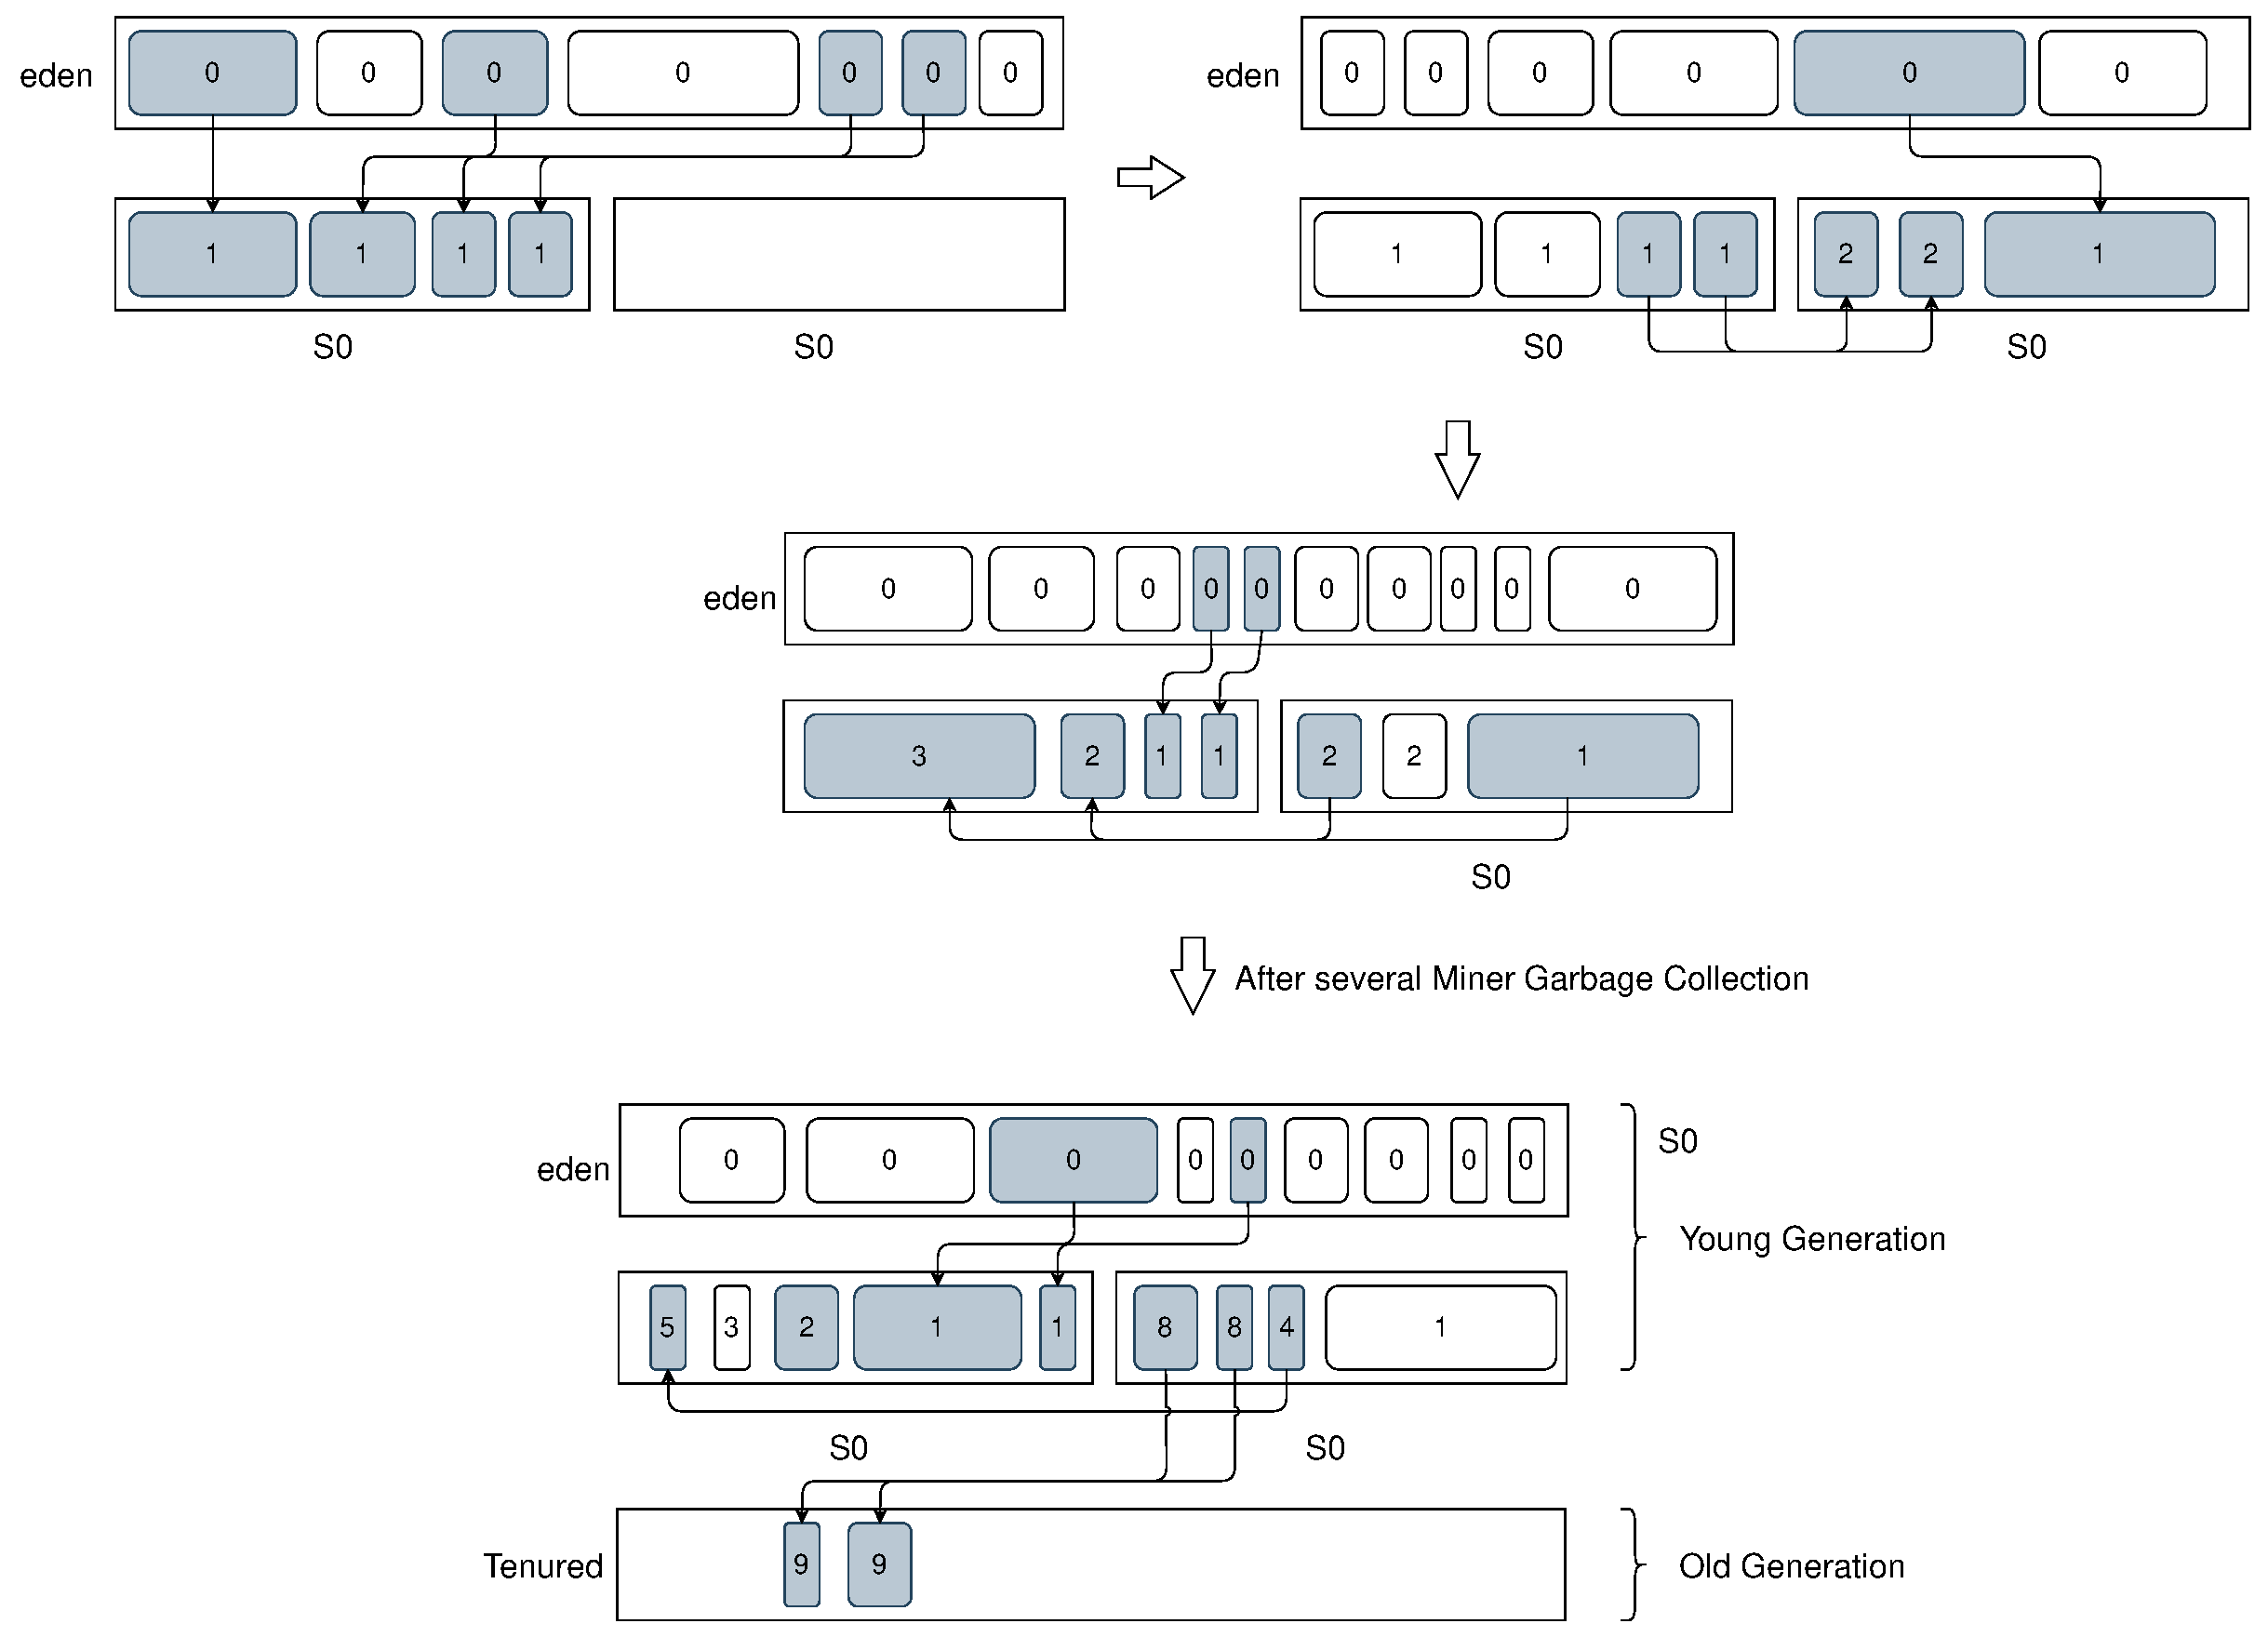
\includegraphics[width=15cm]{java_gc.eps}
    \caption{Java Garbage Collection}
    \label{fig:javagc}
\end{figure}


\subsection{Garbage Collection Tuning}
There are many different ways that one can improve the performance of GC in Java. One of these is for example avoiding pointer-based data structures, such as HashMap and LinkedList. 
These objects have a "wrapper" object for each entry so that number of object tends to be larger than when when an array is used.

Caching serialized object in memory also reduce number of object and memory usage since the set of objects become a byte or binary array. 
Spark SQL applications use DataFrames\cite{DBLP:conf/sigmod/ArmbrustXLHLBMK15}, 
whose intermediate data are managed by an optimized memory manager named Tungsten.
Tungsten stores the intermediate data in a serialized binary form and performs aggregation functions directly on he serialized objects.
Therefore, the number of Java objects in memory is reduced and it reduces the DC frequency and object marking/sweeping. 

In addition, developers can allocate data off-heap of JVM to avoid tracking by GC. 
Facade\cite{DBLP:conf/asplos/NguyenWBFHX15} proposed a compiler and runtime system to bound the number of in-memory data objects, through storing data in an off-heap region and 
manipulating the data with control interfaces.

Although these memory management solution for GC help developer improve performance of Spark applications, 
the effort to discover the best GC tuning afflicts developers.

